\documentclass{standalone}
\usepackage{tikz}
\usetikzlibrary{patterns, positioning}
\usepackage[sfdefault]{ClearSans} %% option 'sfdefault' activates Clear Sans as the default text font
\usepackage[T1]{fontenc}

\begin{document}
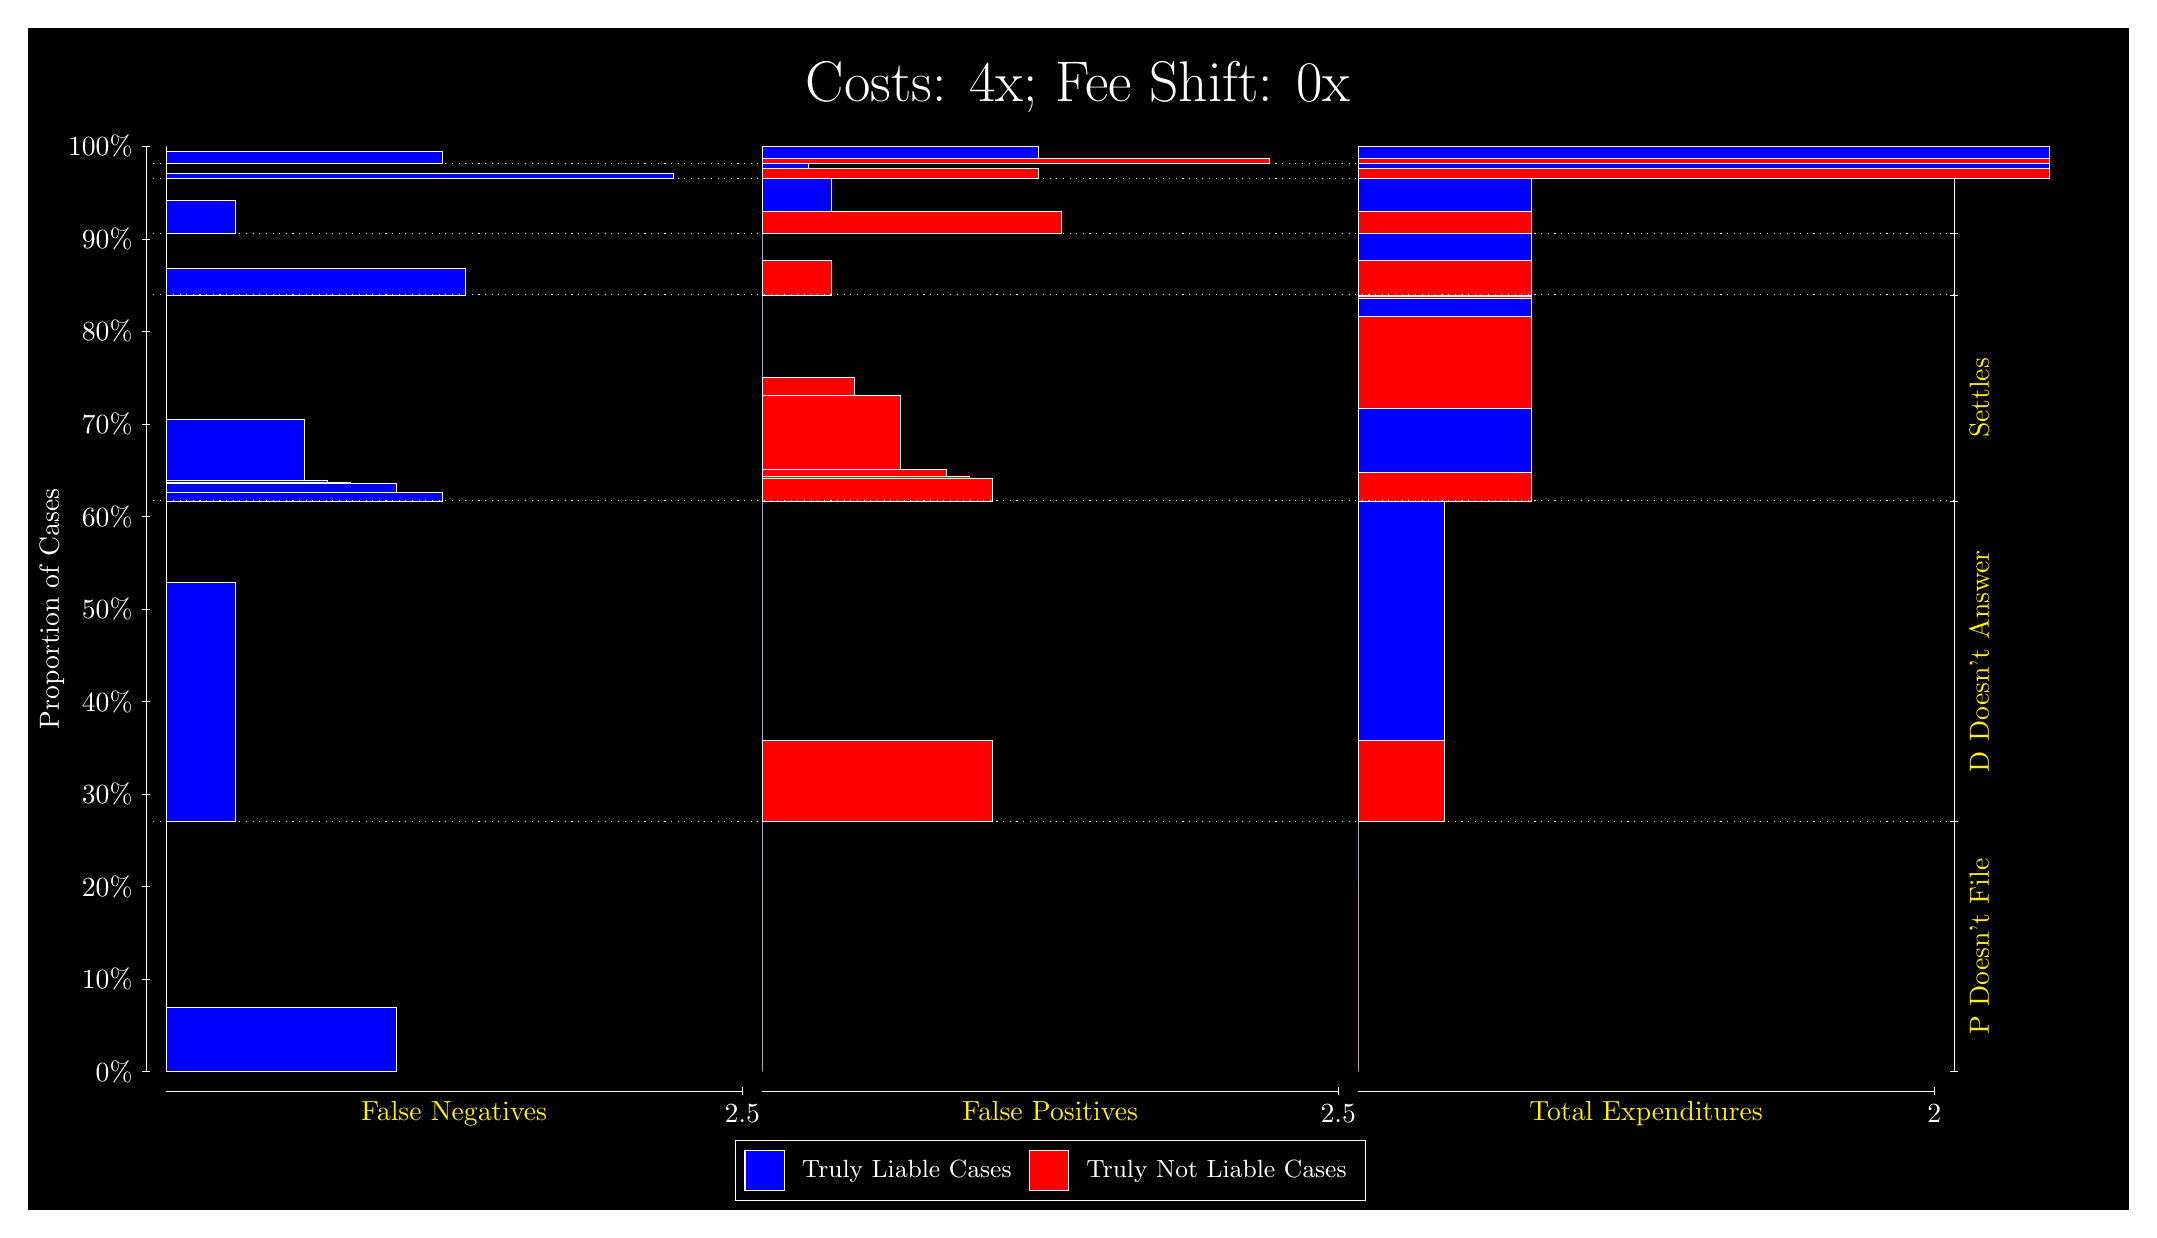
\begin{tikzpicture}
\draw[fill=black] (0,0) rectangle (26.667,15);
\draw[text=white] (0,13.5) rectangle (26.667,15) node[midway] {\huge Costs: 4x; Fee Shift: 0x};
\draw[white, very thin] (1.5,1.75) -- (1.5,13.5);
\node[rotate=90, text=white, anchor=center] at (0.3, 7.625) {Proportion of Cases};
\draw[white, very thin] (1.45,1.75) -- (1.55,1.75);
\node[text=white, anchor=east] at (1.45, 1.75) {0\%};
\draw[white, very thin] (1.45,2.925) -- (1.55,2.925);
\node[text=white, anchor=east] at (1.45, 2.925) {10\%};
\draw[white, very thin] (1.45,4.1) -- (1.55,4.1);
\node[text=white, anchor=east] at (1.45, 4.1) {20\%};
\draw[white, very thin] (1.45,5.275) -- (1.55,5.275);
\node[text=white, anchor=east] at (1.45, 5.275) {30\%};
\draw[white, very thin] (1.45,6.45) -- (1.55,6.45);
\node[text=white, anchor=east] at (1.45, 6.45) {40\%};
\draw[white, very thin] (1.45,7.625) -- (1.55,7.625);
\node[text=white, anchor=east] at (1.45, 7.625) {50\%};
\draw[white, very thin] (1.45,8.8) -- (1.55,8.8);
\node[text=white, anchor=east] at (1.45, 8.8) {60\%};
\draw[white, very thin] (1.45,9.975) -- (1.55,9.975);
\node[text=white, anchor=east] at (1.45, 9.975) {70\%};
\draw[white, very thin] (1.45,11.15) -- (1.55,11.15);
\node[text=white, anchor=east] at (1.45, 11.15) {80\%};
\draw[white, very thin] (1.45,12.325) -- (1.55,12.325);
\node[text=white, anchor=east] at (1.45, 12.325) {90\%};
\draw[white, very thin] (1.45,13.5) -- (1.55,13.5);
\node[text=white, anchor=east] at (1.45, 13.5) {100\%};

\draw[white, very thin] (24.457,1.75) -- (24.457,13.5);
\draw[white, very thin] (24.407,1.75) -- (24.507,1.75);
\node[anchor=west] at (24.407, 1.75) {};
\draw[white, very thin] (24.407,4.9253) -- (24.507,4.9253);
\node[anchor=west] at (24.407, 4.9253) {};
\draw[white, very thin] (24.407,8.9974) -- (24.507,8.9974);
\node[anchor=west] at (24.407, 8.9974) {};
\draw[white, very thin] (24.407,11.613) -- (24.507,11.613);
\node[anchor=west] at (24.407, 11.613) {};
\draw[white, very thin] (24.407,12.393) -- (24.507,12.393);
\node[anchor=west] at (24.407, 12.393) {};
\draw[white, very thin] (24.407,13.096) -- (24.507,13.096);
\node[anchor=west] at (24.407, 13.096) {};
\draw[white, very thin] (24.407,13.284) -- (24.507,13.284);
\node[anchor=west] at (24.407, 13.284) {};
\draw[white, very thin] (24.407,13.5) -- (24.507,13.5);
\node[anchor=west] at (24.407, 13.5) {};

\draw[white, very thin, fill=blue] (1.75,1.75) rectangle (4.6775,2.5681);
\draw[white, very thin, fill=red] (1.75,2.5681) rectangle (1.75,4.9253);
\draw[white, very thin, fill=blue] (1.75,4.9253) rectangle (2.6283,7.9608);
\draw[white, very thin, fill=red] (1.75,7.9608) rectangle (1.75,8.9974);
\draw[white, very thin, fill=blue] (1.75,8.9974) rectangle (5.2631,9.1004);
\draw[white, very thin, fill=blue] (1.75,9.1004) rectangle (4.6775,9.2178);
\draw[white, very thin, fill=blue] (1.75,9.2178) rectangle (4.092,9.2374);
\draw[white, very thin, fill=blue] (1.75,9.2374) rectangle (3.7993,9.2538);
\draw[white, very thin, fill=blue] (1.75,9.2538) rectangle (3.5065,10.037);
\draw[white, very thin, fill=red] (1.75,10.037) rectangle (1.75,11.613);
\draw[white, very thin, fill=blue] (1.75,11.613) rectangle (5.5558,11.954);
\draw[white, very thin, fill=red] (1.75,11.954) rectangle (1.75,12.393);
\draw[white, very thin, fill=blue] (1.75,12.393) rectangle (2.6283,12.818);
\draw[white, very thin, fill=red] (1.75,12.818) rectangle (1.75,13.096);
\draw[white, very thin, fill=blue] (1.75,13.096) rectangle (8.1906,13.156);
\draw[white, very thin, fill=red] (1.75,13.156) rectangle (1.75,13.284);
\draw[white, very thin, fill=blue] (1.75,13.284) rectangle (5.2631,13.441);
\draw[white, very thin, fill=red] (1.75,13.441) rectangle (1.75,13.5);
\draw[white, very thin, fill=red] (9.3189,1.75) rectangle (9.3189,4.1072);
\draw[white, very thin, fill=blue] (9.3189,4.1072) rectangle (9.3189,4.9253);
\draw[white, very thin, fill=red] (9.3189,4.9253) rectangle (12.246,5.9619);
\draw[white, very thin, fill=blue] (9.3189,5.9619) rectangle (9.3189,8.9974);
\draw[white, very thin, fill=red] (9.3189,8.9974) rectangle (12.246,9.2842);
\draw[white, very thin, fill=red] (9.3189,9.2842) rectangle (11.954,9.3137);
\draw[white, very thin, fill=red] (9.3189,9.3137) rectangle (11.661,9.395);
\draw[white, very thin, fill=red] (9.3189,9.395) rectangle (11.075,10.335);
\draw[white, very thin, fill=red] (9.3189,10.335) rectangle (10.49,10.573);
\draw[white, very thin, fill=blue] (9.3189,10.573) rectangle (9.3189,11.613);
\draw[white, very thin, fill=red] (9.3189,11.613) rectangle (10.197,12.052);
\draw[white, very thin, fill=blue] (9.3189,12.052) rectangle (9.3189,12.393);
\draw[white, very thin, fill=red] (9.3189,12.393) rectangle (13.125,12.671);
\draw[white, very thin, fill=blue] (9.3189,12.671) rectangle (10.197,13.096);
\draw[white, very thin, fill=red] (9.3189,13.096) rectangle (12.832,13.225);
\draw[white, very thin, fill=blue] (9.3189,13.225) rectangle (9.9044,13.284);
\draw[white, very thin, fill=red] (9.3189,13.284) rectangle (15.759,13.343);
\draw[white, very thin, fill=blue] (9.3189,13.343) rectangle (12.832,13.5);
\draw[white, very thin, fill=red] (16.888,1.75) rectangle (16.888,4.1072);
\draw[white, very thin, fill=blue] (16.888,4.1072) rectangle (16.888,4.9253);
\draw[white, very thin, fill=red] (16.888,4.9253) rectangle (17.986,5.9619);
\draw[white, very thin, fill=blue] (16.888,5.9619) rectangle (17.986,8.9974);
\draw[white, very thin, fill=red] (16.888,8.9974) rectangle (19.083,9.3656);
\draw[white, very thin, fill=blue] (16.888,9.3656) rectangle (19.083,10.168);
\draw[white, very thin, fill=red] (16.888,10.168) rectangle (19.083,11.346);
\draw[white, very thin, fill=blue] (16.888,11.346) rectangle (19.083,11.567);
\draw[white, very thin, fill=red] (16.888,11.567) rectangle (19.083,11.596);
\draw[white, very thin, fill=blue] (16.888,11.596) rectangle (19.083,11.613);
\draw[white, very thin, fill=red] (16.888,11.613) rectangle (19.083,12.052);
\draw[white, very thin, fill=blue] (16.888,12.052) rectangle (19.083,12.393);
\draw[white, very thin, fill=red] (16.888,12.393) rectangle (19.083,12.671);
\draw[white, very thin, fill=blue] (16.888,12.671) rectangle (19.083,13.096);
\draw[white, very thin, fill=red] (16.888,13.096) rectangle (25.67,13.225);
\draw[white, very thin, fill=blue] (16.888,13.225) rectangle (25.67,13.284);
\draw[white, very thin, fill=red] (16.888,13.284) rectangle (25.67,13.343);
\draw[white, very thin, fill=blue] (16.888,13.343) rectangle (25.67,13.5);
\draw[white, dotted] (1.5,4.9253) -- (24.457,4.9253);
\draw[white, dotted] (1.5,8.9974) -- (24.457,8.9974);
\draw[white, dotted] (1.5,11.613) -- (24.457,11.613);
\draw[white, dotted] (1.5,12.393) -- (24.457,12.393);
\draw[white, dotted] (1.5,13.096) -- (24.457,13.096);
\draw[white, dotted] (1.5,13.284) -- (24.457,13.284);
\draw[white, very thin] (1.75,1.5) -- (9.0689,1.5);
\node[text=yellow, anchor=north] at (5.4094, 1.5) {False Negatives};
\draw[white, very thin] (9.0689,1.45) -- (9.0689,1.55);
\node[text=white, anchor=north] at (9.0689, 1.45) {2.5};

\draw[white, very thin] (9.3189,1.5) -- (16.638,1.5);
\node[text=yellow, anchor=north] at (12.978, 1.5) {False Positives};
\draw[white, very thin] (16.638,1.45) -- (16.638,1.55);
\node[text=white, anchor=north] at (16.638, 1.45) {2.5};

\draw[white, very thin] (16.888,1.5) -- (24.207,1.5);
\node[text=yellow, anchor=north] at (20.547, 1.5) {Total Expenditures};
\draw[white, very thin] (24.207,1.45) -- (24.207,1.55);
\node[text=white, anchor=north] at (24.207, 1.45) {2};

\node[text=yellow, centered, rotate=90] at (24.777, 3.3376) {P Doesn't File};
\node[text=yellow, centered, rotate=90] at (24.777, 6.9613) {D Doesn't Answer};
\node[text=yellow, centered, rotate=90] at (24.777, 10.305) {Settles};





\draw (12.978300999999998,1.5) node[draw=none] (baseCoordinate) {};
\begin{scope}[align=center]
        \matrix[scale=0.5, draw=white, below=0.5cm of baseCoordinate, nodes={draw}, column sep=0.1cm]{
            \node[rectangle, draw, minimum width=0.5cm, minimum height=0.5cm, fill=blue] {}; &
            \node[draw=none, font=\small, text=white] (B) {Truly Liable Cases}; &
            \node[rectangle, draw, minimum width=0.5cm, minimum height=0.5cm, fill=red] {}; &
            \node[draw=none, font=\small, text=white] (B) {Truly Not Liable Cases}; \\
            };
\end{scope}

\end{tikzpicture}
\end{document}